The class SegmentAnalyser offers post-processing methods based on a representation of the plant by segments which connect two nodes with a single line. The segments are derived from the centerlines of the plant organs. We can use this approach to do distributions or calculate densities, and we can analyse the segments within any geometry by cropping the overall geometry to a region of interest. While the class SegmentAnalyser was designed for analysing roots most functionallity works also for the above plant part. 

\subsubsection*{Root surface densities}

We start with a small example plotting the root surface densities of a root system versus root depth.

\lstinputlisting[language=Python, caption= Calculating root surface densities in a soil column]{examples/topics_postprocessing.py}

\begin{itemize}
\item[9-12] Pick a plant or root system.
\item[14-16] Depth is the length of the soil column (into z-direction), layers the number of vertical soil layers, where the root surfaces are accumulated, and runs is the number of simulation runs. 
\item[18] Creates a confing geometry.
\item[20-26] Performs the simulations for $runs$ times. L26 creates a distribution of a parameter (name) over a vertical range (bot, top). The data are accumulated in each layer, segments are either cut (exact = True) or accumulated by their mid point (exact = False). 
\item[28,29] In order to calculate a root surface density from the summed up surface, we need to define a soil volume. The vertical height is the layer length, length and width (here 10 cm), can be determined by planting width, or by a confining geometry. 
\item[30, 31] Calculates the densities mean and the standard error. 
\item[33-42] Prepares the plot (see Figure \ref{fig:topics_postprocessing}).
\end{itemize}

\begin{figure}
\centering
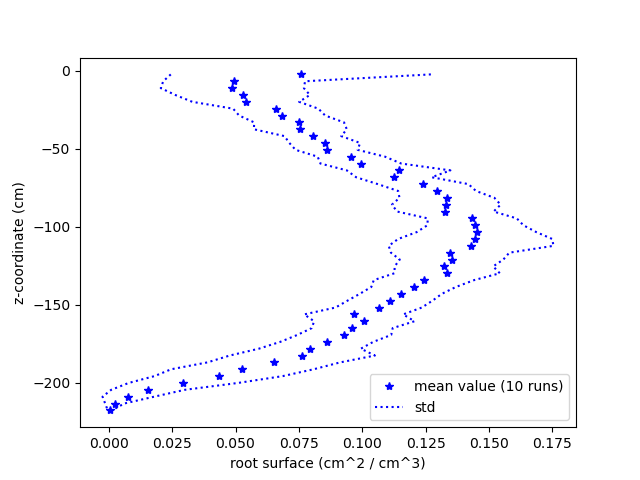
\includegraphics[width=0.7\textwidth]{figures/topics_postprocessing.png} 
\caption{Root surface densitiy versus depth including standard deviation (based on 10 simulation runs) } \label{fig:topics_postprocessing}
\end{figure}




\subsubsection*{Analysis of segment within a cropping geometry}

The following script demonstrates some of the post processing possibilities by setting up a virtual soil core experiment (see Figure \ref{fig:soilcoreGeom}), where we analyse the content of two soil cores located at different positions.

\lstinputlisting[language=Python, caption= A virtual soil core experiment (topics\_postprocessing2)]{examples/topics_postprocessing2.py}

\begin{itemize}
\item[11-15] Performs the simulation.
\item[17-22] We define two soil cores, one in the center of the root and one 10 cm translated. In L22 we pick which one we use for the further analysis. Figure \ref{fig:soilcoreGeom} shows the resulting geometry, with a soil core radius of 10 cm.
\item[24-28] Prepares three sub-figures. 
\item[31-41] Creates a root length distribution versus depth at different ages. L33 creates the SegmentAnalyser object, and L34 crops it to a fixed domain or maps it into a periodic domain. In L38 the filter function keeps only the segments, where the parameter (first argument) is in the range between second and third argument. L39 creates the distribution. 
\item[44-54] We repeat the procedure, but we crop to the soil core selected in L22. 
\item[57-89] In the third sub plot we make densities of specific root types like basal roots, first order roots, and second order roots. In L58 we crop the segments to the soil core geometry. In L63 we filter for the selected sub type, and in L64 we create the density distribution.
\item[71-73] Show and save resulting Figure \ref{fig:central} and \ref{fig:shifted} for the two soil cores (chosen in L22).
\end{itemize}

% \begin{figure}
% \centering
% 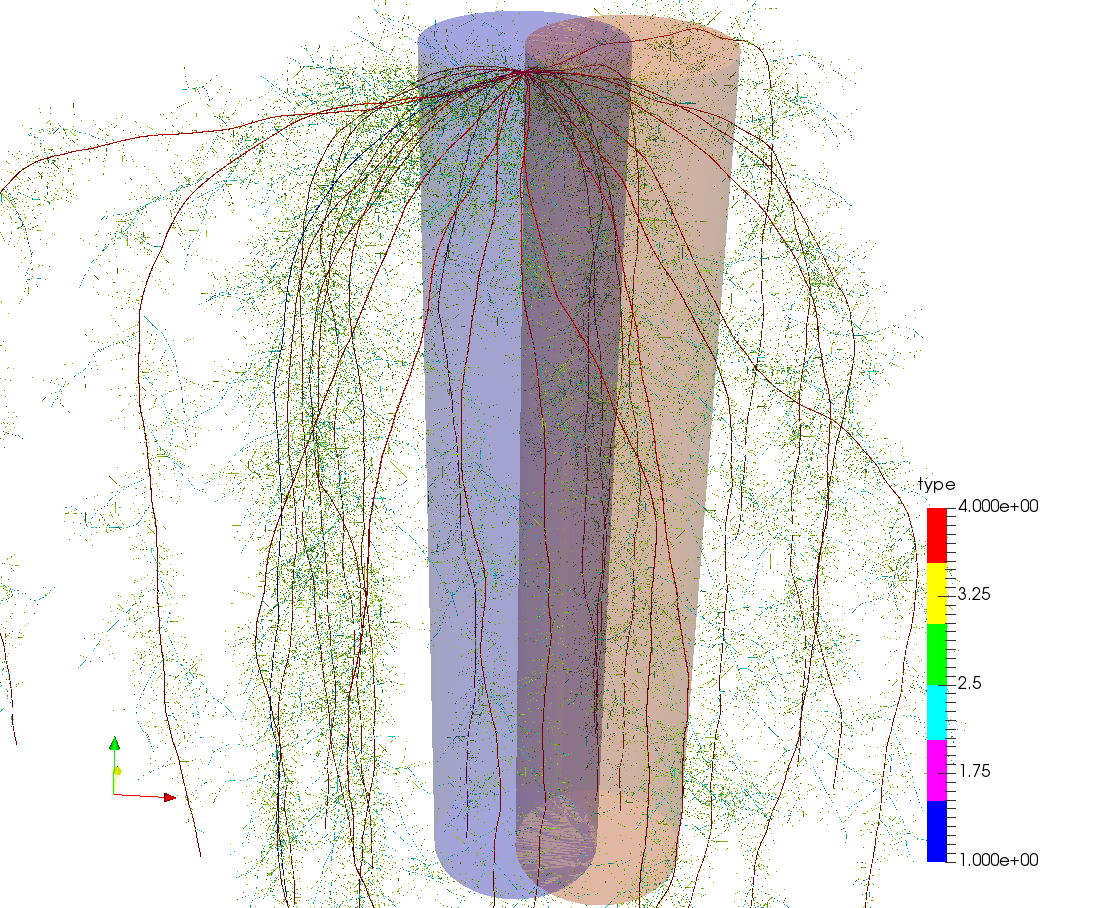
\includegraphics[width=0.7\textwidth]{example_3d.png} % 
% \caption{Virtual soil cores experiment (Example 3b): Central core (blue), shifted core (red)} \label{fig:soilcoreGeom}
% \end{figure} 


The example shows differences between the central core and shifted core (see Figure \ref{fig:central} and \ref{fig:shifted}) because the central core captures all roots emerging from the seed. The basic idea is that such analysis can help to increase the understanding of variations in experimental observations.
% 
% \begin{figure}
% \centering
% 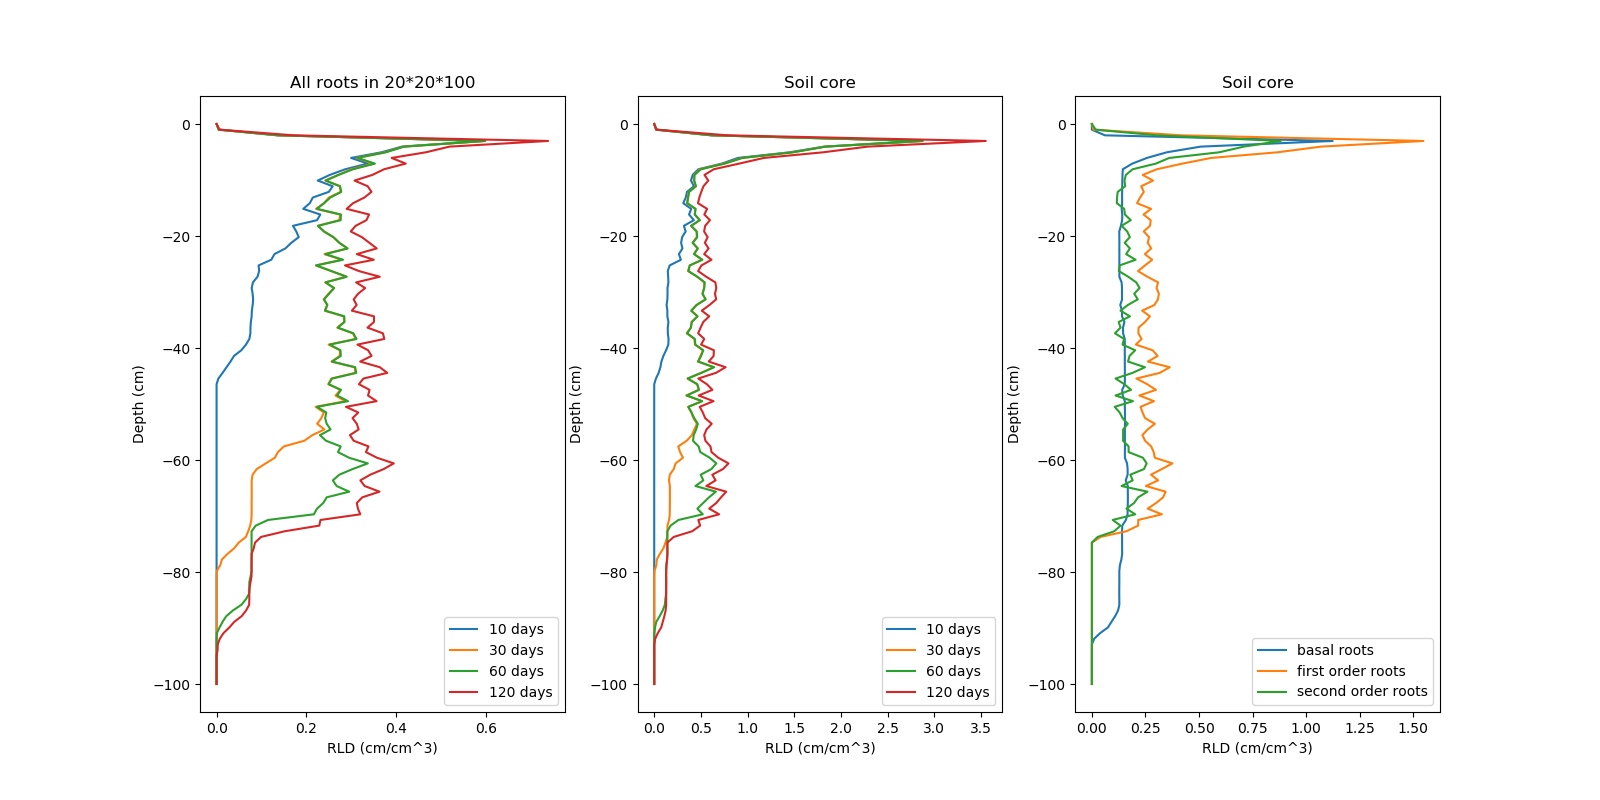
\includegraphics[width=0.9\textwidth]{example3b.png} 
% \caption{Central core (Example 3b)} \label{fig:central}
% \end{figure}
% 
% \begin{figure}
% \centering
% 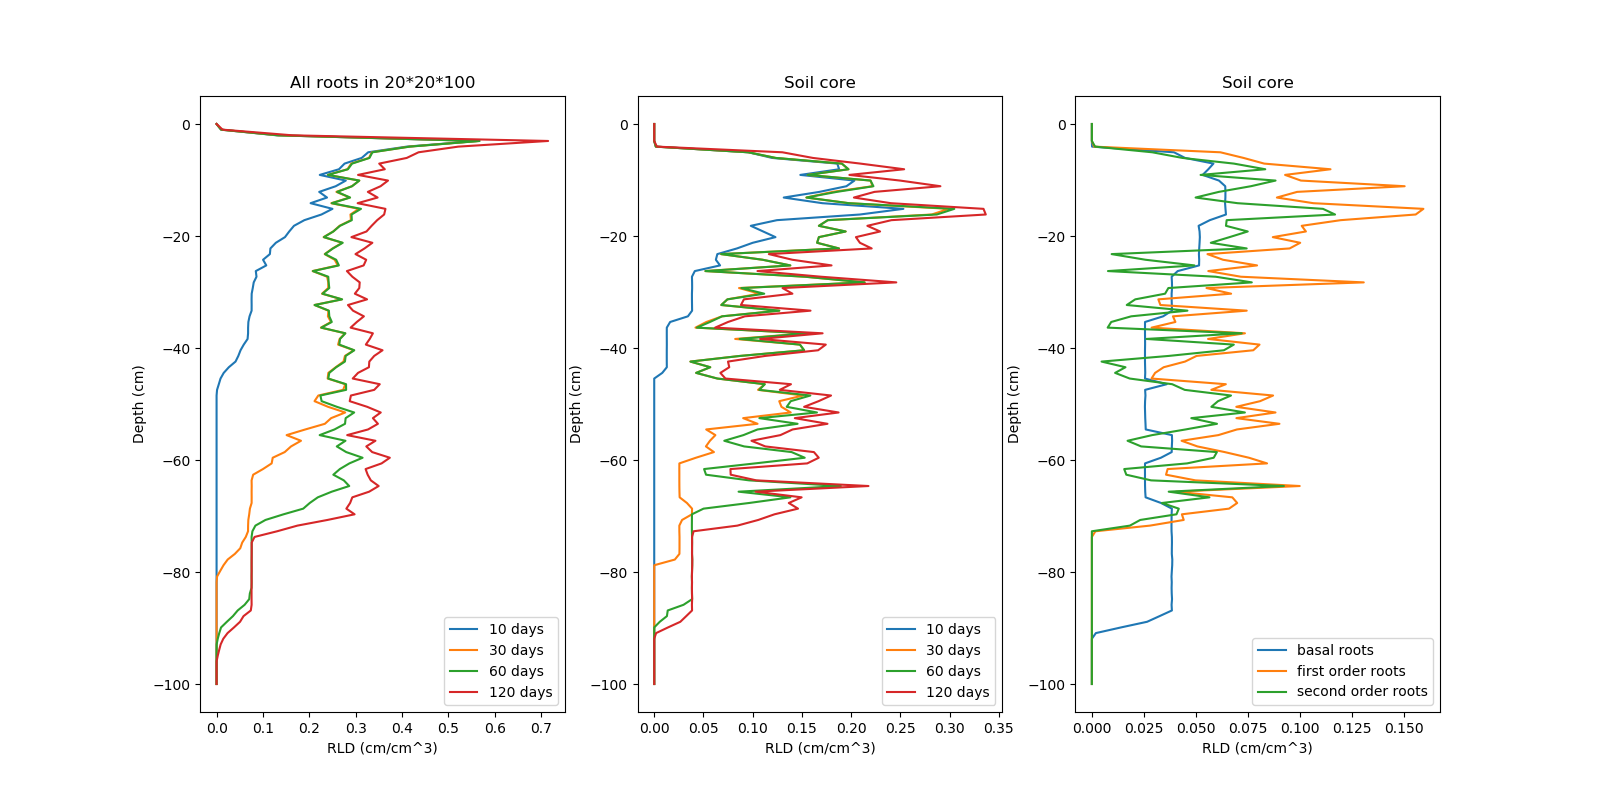
\includegraphics[width=0.9\textwidth]{example3b2.png} 
% \caption{Shifted core (Example 3b)} \label{fig:shifted}
% \end{figure}


\subsubsection*{SegmentAnalyser for measurements}

It is also possible to make use of the SegmentAnalyser class without any other CPlantBox classes (e.g. for writing vtp from measurements). The following example shows how to construct the class with arbitrary nodes and segments (e.g. from measurements). 

\lstinputlisting[language=Python, caption=SegmentAnalyser can be used on measured data (topics\_postprocessing3.py) ]{examples/topics_postprocessing3.py}

\begin{itemize}
 \item[7-11] Define some segments with data
 \item[14,15] We convert the Python list to lists of C++ types
 \item[18] We create the SegmentAnalyser object without an underlying plant
 \item[19,20] Use the Analyser object, by printing information, or writing a vtp. 
 \item[21] Visualize your results
\end{itemize}
